\documentclass{sig-alternate}

\usepackage{algorithmic}
\usepackage{algorithm}
\usepackage{amsmath,amssymb}
\usepackage{stmaryrd}
\usepackage{graphicx}
\usepackage{color}

\DeclareGraphicsRule{.tif}{png}{.png}{`convert #1 `dirname #1`/`basename #1 .tif`.png}

\newcommand{\longversion}[1]{}
\newcommand{\comment}[1]{}
\newcommand{\tinysection}[1]{\vspace{0.5mm}\noindent{\bf #1.}}
\newcommand{\tuple}[1]{{\langle#1\rangle}}
\newcommand{\todo}[1]{[\textcolor{red}{#1}]}
\newcommand{\note}[1]{[\textcolor{blue}{#1}]}
\newcommand{\dbtoaster}[0]{[ANONYMIZED]}

\newtheorem{example}{Example}[section]

\toappear{}

\title{Multilevel Incremental View Maintenance and the Confluence of
Compilers and Query Optimizers}
%\numberofauthors{3}
\numberofauthors{1}
\author{
%\alignauthor
%Yanif Ahmad\\
%    \affaddr{Johns Hopkins University}
%    %\affaddr{Baltimore, MD}
%    \email{yanif@cs.jhu.edu}
%\alignauthor
%Oliver Kennedy\\
%    %\affaddr{\'Ecole Polytechnique F\'ed\'erale de Lausanne} \\
%    \affaddr{EPFL}
%    %\affaddr{Lausanne, Switzerland}
%    \email{oliver.kennedy@epfl.ch}
%\alignauthor
%Christoph Koch\\
%    \affaddr{EPFL}
%    % \affaddr{\'Ecole Polytechnique F\'ed\'erale de Lausanne} \\
%    %\affaddr{Lausanne, Switzerland}
%    \email{christoph.koch@epfl.ch}
}


\begin{document}
\maketitle


\begin{abstract}
Multilevel incremental view maintenance generalizes the idea of using materialized views for query answering by allowing a query optimizer to also use materialized views for answering delta queries, that is, the auxiliary queries that are used to refresh materialized views when updates happen. Aggressive recursive use of this idea can allow to eliminate all joins from certain queries, yielding the option of generating highly efficient low-level code without classical query operators that performs all query evaluation and view refreshment work. This calls for the compilation of queries.

In this paper, we present a general compiler architecture for database queries and multi-level incremental view maintenance which is applicable to languages such as SQL. To realize such a compiler, we overcome the challenges of materializing views with binding patterns (parameters) to support arbitrarily nested queries with aggregates, complex patterns of side effects that may arise, and the need to perform sophisticated forms of deforestation and fusion popular and essential in compilers but almost unknown in the database literature.

Aggressive multilevel incremental view maintenance bears the potential to be, by many degrees of magnitude, faster than classical incremental view maintenance and to have substantially greater expressive power compared to the query languages supported in stream engines; this may lead to a new breed of data management systems that can drive sophisticated streaming, online, and real-time analytics that are not supported by current data management systems.
We illustrate this through extensive experimentation with different parameterizations of our compiler as well as existing DBMS and stream engines, on an analytics workload composed of monitoring, algorithmic trading, and ETL queries. 
\end{abstract}


\section{Introduction}
\label{sec:introduction}
\section{Introduction}


Recent years have seen the beginning of a paradigm shift in data management
research from incrementally
improving decades-old database technology
%
% (particularly, OLTP) -- System R and
% the long line of systems that have followed it --
%
to questioning established
architectures and creating fundamentally different, more lightweight systems
that are often domain-specific
(cf.\ e.g. \cite{DBLP:conf/vldb/StonebrakerMAHHH07,DBLP:journals/pvldb/KallmanKNPRZJMSZHA08}).
Part of the impetus for this change was given by 
potential users such as scientists and the builders of
large-scale Web sites and services such as Google, Amazon, and Ebay,
who have a need for data management systems but have found current databases
not to scale to their needs.
One can observe a trend to disregard database contributions
in these communities \cite{dbcolumn, DBLP:conf/sigmod/PavloPRADMS09}, and to build lightweight systems based on
robust technologies mostly pioneered by the operating systems and distributed
systems communities, such as large scale file systems, key-value stores, and
map-reduce
\cite{DBLP:journals/cacm/DeanG08, DBLP:journals/tocs/ChangDGHWBCFG08}.
Further impetus has resulted from the current need to develop data management
technology for multicore and cloud computing.
%
%, and by the example given by a
%number of innovative recent database startup companies that develop
%databases based on new architectures.
%\footnote{Examples are Vertica and Paraccel, who build column stores,
%and Greenplum, Asterdata, and Netezza, who take databases into the Cloud.}

There is a recent tendency among pundits outside the database community to
contest the need for powerful queries, and to
think of key-value stores -- with only the power to look up data by
keys -- as (much more efficient) database query engines.
%
%It shall not be denied that,
%with clever engineering, a surprising range of problems can be solved
%using key-value stores.
%
However, expressive query languages such as SQL do not cease to have
important applications and a substantial user base.
Alas, we do not know how to process SQL queries on updateable data
using a system as lightweight as a key-value store.

This paper contributes a fundamental and versatile building block for
enabling new, more lightweight and nimble data processing systems based
on SQL aggregation que\-ries. We believe that our contribution
constitutes an important
step towards achieving the contradiction in terms mentioned
above: executing complex aggregation queries on updateable data
using little more than a key-value store.

At the heart of our approach is a new aggressive recursive incremental
view maintenance mechanism.
In most traditional database query processors, the  basic building blocks of
queries are large-grained operators such as joins.
Our approach is based on compilation, reducing
queries to programs that are not based on classical query operators.
A large class of
SQL aggregation queries can be compiled down to very simple message
passing programs that incrementally maintain materialized views of
the queries. These message passing programs keep a hierarchy of map data
structures (which may be served out of a key-value store) up to date
and can share computation in the case that multiple aggregation queries (e.g.,
a data cube) need to be maintained.  Most importantly, though, these message
passing programs can be massively parallelized to the degree that the updating
of each single result aggregate value can be done in constant time on normal
off-the-shelf computers.\footnote{That is,
we assume that addition and multiplication
of {\em two numbers} can be performed in constant time, which is true for
%
%bounded precision numbers such as 
%
standard base types such as int and float,
but we assume no unrealistic models such
as aggregators with unbounded fan-in, as used in some theoretical models of
parallel computation. Our implementation indeed incrementally maintains
individual aggregate values in constant time. Note that since there are
usually many more aggregate values to maintain than there are processors,
this does not mean that each update is processed in constant time.
``Constant time'' is with respect to the size of the data, not the compiled
query.}
To the best of our knowledge, it was not known before
that this is possible.

In comparison, no such constant-time parallel processing technique
is known for nonincremental query
evaluation: Indeed, it is unlikely to exist.\footnote{Constant-time
bounded fan-in nonincremental
parallel processing is known not to be possible for
the class of queries we address,
unless the complexity class TC0 collapses into NC0, which it is not known
to do \cite{Joh90}.} Classical incremental view maintenance approaches, which
express the delta (=change) to a query result given an update again
as a (slightly simpler) query, fare no better: Generally,
given a query, there is another query whose delta is the first query.
Thus, classical incremental view maintenance has the same limits to
parallelization as nonincremental evaluation.


\subsection{Message passing programs}


We compile SQL aggregation queries to {\em map maintenance
message}\/ (M3) programs. An M3 program consists of a set of triggers of
the form
\[
\mbox{{\tt on insert into $R$($\vec{x}$) \{
($\vec{y}$:$D_{\vec{y}}$) $m[\vec{x}, \vec{y}]$ += $s$
\}}}
\]
or
\[
\mbox{{\tt on delete from $R$($\vec{x}$) \{
foreach $\vec{y}$ do $m[\vec{x}, \vec{y}]$ -= $s$
\}}}
\]
where $R$ is a relation name,
$\vec{x}$ and $\vec{y}$ are distinct tuples of variables and
$s$ is either a term or of the form
{\tt if $\phi$ then $t$ else 0}, where $t$ is a term.
Terms are built from addition, multiplication,
constants, variables from $\vec{x}$, external function calls $f(\vec{z})$,
and map accesses $m_1[\vec{z}_1], \dots, m_k[\vec{z}_k]$ where
$m$, $m_1$, $\dots$, $m_k$ are pairwise distinct
and the variables in $\vec{z}_1, \dots, \vec{z}_k$ are a nonoverlapping
subsets of the variables in $\vec{x}, \vec{y}$.
Conditions $\phi$ are conjunctions of comparisons $t'' \;\theta\; t'''$,
where $t'',t'''$ are terms without map accesses and
$\theta \in \{ =,<,\le,\neq \}$.
If $\vec{y}$ consists of zero variables, we omit
{\tt foreach $\vec{y}$ do}.
For each relation name, there may by multiple insert and delete triggers.

M3 programs can be read as straightforward pseudocode.
There are subtle issues to be discussed later about the domains of 
variable tuples
to be iterated over by foreach loops. Let us for now assume that
{\tt foreach $\vec{x}$ do $(\dots)$} iterates over all distinct tuples of
values currently in the
database, and that map values $m[\vec{x}]$ for $\vec{x}$ containing newly
inserted values are initially zero.


\begin{example}\em
\label{ex:TPCH-Q12}
Consider the following query on a TPC-H like schema,
which counts the number of LineItems per customer id.
\begin{verbatim}
SELECT   C.cid, SUM(1)
FROM     Customer C, Order O, LineItem L
WHERE    C.cid=O.cid AND O.oid=L.oid
GROUP BY C.cid;
\end{verbatim}
Here, cid is a key for the Customer relation and oid is a key for the
Order relation, but oid is not a key for LineItem.
Our compiler translates this query to the M3 program
\begin{verbatim}
on insert into Customer (cid, ...) { qO1[cid] += 1 }
on insert into Order (oid, cid, ...) {
  qL[cid, oid] += qO1[cid]
}
on insert into LineItem (oid, ...) {
  foreach cid do q[cid] += qL[cid, oid]
}
\end{verbatim}

In this and the following example, the delete-triggers are precisely
like the insert-triggers, but with {\tt +=} replaced by {\tt -=}.
Thus, to save space, the deletion triggers are omitted.

Let us ignore parallelization first.
It is not hard to see that this trigger program correct maintains the
query result, for each distinct {\tt cid} in Customer.cid, as {\tt q[cid]}.
(The maps {\tt qO1} and {\tt qL} are auxiliary.)
We assume that
there are no cascading deletes and, for instance, before we can delete an
Order, we have to delete all associated lineitems.
\punto
\end{example}


{\em Parallelization}.
The syntax of statements
\begin{equation}
\mbox{{\tt foreach $\vec{y}$ do $m[\vec{x}, \vec{y}]$ $\pm$= $s$}}
\label{eq:foreach}
\end{equation}
is misleading in that it suggests a loop --
that a nonconstant amount of work is needed to bring aggregate
values up to date. Of course, polynomial amounts of work are in fact need,
but only because in general there are many aggregate values -- in a
map representing the result of a group-by query or in an auxiliary map --
to be maintained. In fact, each statement of form (\ref{eq:foreach})
writes each value $m[\vec{x}, \vec{y}]$ only once and admits
{\em embarassing parallelism}: $m$ can be partitioned across many machines
that share the work.

Assume that the storage of individual maps
is partitioned across several machines. To execute a statement of form
(\ref{eq:foreach})
in a trigger invocation with arguments $\vec{x} = \vec{a}$,
where $s$ uses map lookups $m_i[\vec{x}_i, \vec{y}_i]$,
each node storing a value $m_i[\vec{a}_i, \vec{y}_i] = v$,
for $\vec{y}_i$ arbitrary, sends the message
$m_i[\vec{a}_i, \vec{y}_i] = v$ to the node managing value
$m[\vec{a}, \vec{y}]$. This way, that node receives all the values it
needs to update all $m$ values it represents.
Of course this requires a suitable protocol to ensure overall consistency
and that the right versions of map values are read and written in the right
order.



\begin{example}[star-join decomposition]\em
\label{ex:ssb}
Con\-sider \\ a simplified version of the star schema
benchmark (SSB) schema with relations Date(\underline{datekey}, year),
Part(\underline{partkey}, partcat), where partcat stands for a part category,
and LineOrder(datekey, partkey, revenue), which may contain duplicate tuples.
The query asks for the total revenues grouped by year and part category.

\begin{verbatim}
SELECT   P.partcat, D.year, SUM(revenue)
FROM     Date D, Part P, LineOrder L
WHERE    D.datekey=L.datekey
AND      P.partkey=L.partkey
GROUP BY P.partcat, D.year;

on insert into Date (datekey, year) {
  mPL[datekey, year] += 1
}
on insert into Part (partkey, partcat) {
  mDL[partkey, partcat] += 1
}
on insert into LineOrder (datekey, partkey, revenue) {
  foreach (partcat, year) do
  m[partcat, year] += revenue
                    * mDL[partkey, partcat]
                    * mPL[datekey, year]
}
\end{verbatim}

Observe how, on insertion into LineOrder, the code for incrementally
maintaining the query result {\tt m} decomposes into
two parts with disjoint variables, 
{\tt mDL[partkey, partcat]} and {\tt mPL[datekey, year]}.

The maps mPL and mDL have value at most
one at each position because datekey and partkey are keys for Date and Part,
respectively.

On insert into LineOrder, given values for
datekey and partkey, we instruct nodes
to send their {\tt mDL[partkey, x]} and {\tt mPL[datekey, y]} values,
for any {\tt x} and {\tt y},
to nodes maintaining {\tt m[x, *]} and {\tt m[*, y]}, respectively.
A node managing {\tt m[u, v]} receives, possibly from distinct nodes,
{\tt mDL[partkey, u]} and {\tt mPL[datekey, v]}
and can increment {\tt m[u, v]} by
{\tt revenue*mDL[partkey, u]*mPL[datekey, v]}.
%
%We only send nonzero {\tt mDL[partkey, x]} and {\tt mPL[datekey, y]} values,
%but at least an empty message so that the node managing m knows that it does
%not have to wait for anything more.
\punto
\end{example}


\begin{example}[self-join]\em
\label{ex:self-join}
We now ask, for each customer id (cid),
for the number of customers of the same nation (including the customer
identified by cid in the count).
\begin{verbatim}
SELECT   C1.cid, SUM(1)
FROM     Customer C1, Supplier C2
WHERE    C1.nation = C2.nation
GROUP BY C1.cid;
\end{verbatim}
The compiler produces the following on-insert trigger:
\begin{verbatim}
on insert into Customer (cid, nation) {
  q[cid] += qC1[nation];
  foreach cid2 do q[cid2] += qC2[cid2, nation];
  q[cid] += 1;
  qC1[nation] += 1;
  qC2[cid, nation] += 1
}
\end{verbatim}
The on-delete trigger is just like the on-insert trigger with {\tt +=}
changed to {\tt -=} everywhere other than in the third statement
({\tt q[cid] += 1}), which remains unchanged.
We will establish later that this M3 program is indeed correct.

For now, we challenge the reader to find a 
fundamentally different (ideally, simpler) way to
perform the incremental maintenance of {\tt q}
which has the M3 property of embarassing parallelism, with each value
to be updated only requiring a constant amount of work.
Examples~\ref{ex:TPCH-Q12} and \ref{ex:ssb} were chosen for simplicity,
but we believe that this example shows that creating M3 programs in general
is nontrivial.
\punto
\end{example}


It shall be emphasized that for each of the examples of this section,
and the paper as a whole, our compilation approach produces exactly
the M3 programs shown.


The fragment of SQL queries that we can compile to M3 essentially comprises
SUM-agg\-regation queries with group-by.
COUNT and AVG queries can be defined by arithmetic expressions over these.
We exclude MIN and MAX queries, aggregation
nested into FROM or WHERE clauses, the DISTINCT and HAVING keywords,
outerjoins,
and the relational difference operation. At the end of this paper, we will
discuss which of these features can be added without fundamental difficulties.


\subsection{The Cumulus System}


We have developed a system, Cumulus\footnote{A Cumulus cloud is an
aggregation cloud, thus the name.}, that parallelizes the
execution of M3 programs in a cluster or computing cloud.
Cumulus performs incremental maintenance of exact aggregation views online, and
executes an efficient
protocol to ensure consistency of map data and query results,

While it is no fundamental requirement of our compilation
approach, we have chosen to use the resources of the cloud to maintain
the data in main memory, allowing for very low latency updating and querying.
At the time of writing this,
Terabyte-sized memory chips (DIMMs and flash) have already been announced by
manufacturers, and already now, large data warehouses
can be run in main memory in the cloud, where additional hardware costs
(main memory is more expensive per TB than hard disks) are
offset by greater robustness of the system, lower maintenance
costs, lower heat production \cite{1154557}, and of course by of orders
of magnitude better speed and latency characteristics.

The Cumulus protoype aims at demonstrating our results in the context of
pushing OLAP into the cloud.
Cumulus automates  the process of  creating, loading,
and  maintaining  in-memory  data  warehouses.
(Optional logging of updates to secondary storage
for persistency is supported.)
Cumulus targets OLAP applications  that perform real-time analytics of
relational data.  By feeding it an SQL query, Cumulus's infrastructure
becomes linked to  a set of OLTP databases.  Cumulus  keeps the
data warehouse synchronized with the source databases via an
update stream. It achieves synchronization {\em in realtime}
through parallelization, keeping data in main memory, and our approach of
query processing by message passing.


\subsection{Contributions and Structure of the Paper}


Our main technical contributions are as follows.
\begin{itemize}
\item
We present M3, a massively parallelizable language
for message passing programs that can be used to incrementally maintain
SQL aggregation queries.

\item
We describe our compiler for translating SQL aggregation queries to M3
programs. Our compilation technique is based on a novel, aggressive, recursive
form of incremental view maintenance.

\item
We present Cumulus, our system for exact online aggregation in realtime.
We describe the Cumulus message passing protocol, which assures
consistency of the maps using only few messages, and
infrastructure, and show how it can be used to efficiently distribute the
processing and storage requirements of query processing and
the incremental maintenance of large aggregate views and datacubes.

\item We show evidence for the scalability of our approach by examining the
performance of Cumulus on examples drawn from the TPC-H\cite{tpch2008}
benchmark. 
\end{itemize}


The remainder of this paper is organized as follows.
Section \ref{sec:compiler} describes our SQL to M3 compiler.
In Section \ref{sec:architecture}, we provide an overview of Cumulus's online
infrastructure and discuss how data is managed within that infrastructure.
Section \ref{sec:experiments} presents
experimental results that demonstrate the viability and scalability of
Cumulus.
Section \ref{sec:relatedwork} discusses related work.
The paper concludes with Section \ref{sec:conclusions}






\section{Motivation and Related Work}
\label{sec:dbfail}
\subsection{The Challenges of Monitoring}
Consider the following examples of commonplace automated tasks in three different application domains:
\begin{enumerate}
\item An automated stock market trading system monitors the distribution of buy and sell orders of a particular stock to identify the best time and price for its own orders.
\item A corporate data warehouse monitors the current status of its production facilities, warehoused inventory and active demand for its products in order to preemptively identify supply chain problems.
\item A compute cluster monitors its current status overnight to alert a network administrator when some of its hardware fails, but only if the chance of computations being disrupted by further failures exceeds a given threshold.
\end{enumerate}

The core challenge in automating each of these tasks is the instantiation of a system for {\em monitoring} the state of the world from the application domain's perspective, be it a stock market, data warehouse, or compute cluster, etc\ldots.  This is a fundamentally data-management challenge: As the state of the world changes, the monitoring system must update it's own internal view of that state accordingly -- each order placed for a given stock can potentially affect the automated trading system's behavior.  

In spite of this, the challenges associated with monitoring rapidly changing, but otherwise persistent state have not been sufficiently addressed by the database community. Although active database (i.e., Triggers)\cite{?} and complex stream event processing (CEP)\cite{?} techniques both address the challenges of monitoring persistent state, neither is designed to handle complexity in the monitoring task, nor rapid changes to ``persistent'' state.  In this section we now support this assertion through experimental (and some anecdotal) evidence, which clearly demonstrates that existing data-management systems are incapable of efficiently performing these sorts of monitoring tasks.

We consider the three example scenarios as described above.  Each monitoring task is implemented using triggers in Postgres and two commercial database systems, and using CEP in two commercial stream processing systems\footnote{The names of the commercial databases and stream processors are kept anonymous due to restrictions in their license agreements.}.  Concretely, the scenarios are as follows:

\begin{figure}
\tinysection{Example \ref{ex:dbfail:stock}}
\begin{verbatim}
-- Example 2.1 --
CREATE TABLE bids(volume float, price float);
CREATE TABLE asks(volume float, price float);
\end{verbatim}

\tinysection{Example \ref{ex:dbfail:tpch}}'s schema is identical to the TPC-H schema\cite{tpch}.

\tinysection{Example \ref{ex:dbfail:network}}
\begin{verbatim}
CREATE TABLE Server(ssid int, status int);
CREATE TABLE Task(ttid int, priority int);
CREATE TABLE Assignment(asid int, atid int);
\end{verbatim}

\label{fig:dbfail:schemas}
\caption{Schemas for the three example scenarios}
\end{figure}

\begin{example}
\label{ex:dbfail:stock}
A stock market trading system monitors the spread across significant orders for a particular stock (i.e., orders larger than 0.01\% of the total volume of orders for the stock).  Given the table schemas defined in Figure \ref{fig:dbfail:example:schemas}, we can express the value being monitored as a SQL query:
% test/sql/finance/pricespread.sql
\begin{verbatim}
SELECT SUM(a.price - b.price)
FROM   bids b, asks a
WHERE  b.volume > 0.0001 * (SELECT SUM(b1.volume) 
                            FROM   bids b1)
  AND  a.volume > 0.0001 * (SELECT SUM(a1.volume) 
                            FROM   asks a1);
\end{verbatim}
\end{example}

\begin{example}
\label{ex:dbfail:tpch}
A corporate data warehouse monitors the volume of of parts of each type being shipped between each region based on the locations of the supplier and the client.  Given the standard TPC-H benchmark schema\cite{tpch}, we can express this monitoring task as the following SQL group-by query (based on, but not identical to SSB query 4\cite{ssb}): 
\begin{verbatim}
SELECT   sn.regionkey, cn.regionkey,
         p.type, SUM(li.quantity)
FROM     CUSTOMER c, ORDERS o, LINEITEM li, PART p, 
         SUPPLIER s, NATION cn, NATION sn
WHERE       c.custkey = o.custkey
  AND      o.orderkey = li.orderkey
  AND       p.partkey = li.partkey
  AND       s.suppkey = li.suppkey
  AND    cn.nationkey = c.nationkey
  AND    sn.nationkey = s.nationkey
GROUP BY sn.regionkey, cn.regionkey, PART.type;
\end{verbatim}
\end{example}

\begin{example}
\label{ex:dbfail:network}
A cluster monitoring system keeps monitors servers assigned to work on different compute tasks -- the system issues an alert whenever the number of failed servers assigned to a given task exceeds a given threshold (e.g., 50\%).  These alerts are dispatched based on priority, and number of threatened tasks.  Given the table schemas defined in Figure \ref{fig:dbfail:example:schemas}, we can represent this monitoring task as triggering whenever the following SQL group-by query returns a non-empty result:
\begin{verbatim}
SELECT priority, COUNT(*)
FROM   Task t
WHERE  (SELECT COUNT(*) 
        FROM Assignment a2,Server s2
        WHERE t.ttid = a2.atid 
        AND a2.asid = s2.ssid) * 0.5 > 
       (SELECT COUNT(*) 
        FROM Assignment a3,Server s3
        WHERE t.ttid = a3.atid 
        AND a3.asid = s3.ssid 
        AND s3.status = 1)
GROUP BY t.priority;
\end{verbatim}
\end{example}

\subsection{Monitoring with Active Databases}
The first existing technique for monitoring in the database literature is based around so called Active Databases\cite{?}.  This technique allows user-defined {\em triggers} to intercept updates to one table in the database, and initiate secondary updates as a result.  Trigger functionality has been implemented in most high-end database management systems -- Postgres\cite{?}, MySQL\cite{?}, and virtually all commercial systems, including the two we test.

Closely related to Active Databases are Incremental View Maintenance\cite{?} (IVM) systems.  Rather than allowing arbitrary user-defined operations to trigger after updates to the database, IVM systems allow users to define materialized views.  The result of the view query is materialized, but rather than re-evaluating the entire query from scratch whenever one of the tables in the query changes, the IVM system uses a so-called delta query.  The delta query is a simpler form of the original query, which identify how the original query changes as after an update to one of its tables.  

\begin{example}
For example, consider the query from Example \ref{ex:dbfail:tpch} and an insertion into the {\tt LINEITEM} table:
\begin{verbatim}
INSERT INTO 
LINEITEM(orderkey, partkey, suppkey, quantity)
VALUES  (37,       42,      7,       100);
\end{verbatim}

We can run the following query:
\begin{verbatim}
SELECT   sn.regionkey, cn.regionkey,
         p.type, SUM(100)
FROM     CUSTOMER c, ORDERS o, PART p, 
         SUPPLIER s, NATION cn, NATION sn
WHERE       c.custkey = o.custkey
  AND      o.orderkey = 37
  AND       p.partkey = 42
  AND       s.suppkey = 7
  AND    cn.nationkey = c.nationkey
  AND    sn.nationkey = s.nationkey
GROUP BY sn.regionkey, cn.regionkey, PART.type;
\end{verbatim}

Note that all columns from {\tt LINEITEM} have been replaced by the corresponding value being inserted.  The result of running this query is the delta to the original table.  The delta is then merged into the original query's materialized results -- group by terms are paired with like values from the original query, and the new sums are added to the corresponding old ones.  After merging in the delta, the materialized view correctly represents the results of the original query after the insertion into {\tt LINEITEM}.
\end{example}

Because the delta query is simpler, it can be evaluated more efficiently than the original, conceivably saving time on updates.  IVM functionality has been implemented into most commercial database systems, including the two we test.

\begin{figure*}
\begin{center}
\begin{tabular}{ccc}
\includegraphics[width=2in]{../graphics-tmp/placeholder_db_result} &
\includegraphics[width=2in]{../graphics-tmp/placeholder_db_result} &
\includegraphics[width=2in]{../graphics-tmp/placeholder_db_result} \\
(a) & (b) & (c)
\end{tabular}
\end{center}
\label{fig:dbfail:postgres}
\caption{Performance results for Postgres on Examples \ref{ex:dbfail:stock} (a), \ref{ex:dbfail:tpch} (b), and \ref{ex:dbfail:network} (c).}
\end{figure*}
\begin{figure*}
\begin{center}
\begin{tabular}{ccc}
\includegraphics[width=2in]{../graphics-tmp/placeholder_db_result} &
\includegraphics[width=2in]{../graphics-tmp/placeholder_db_result} &
\includegraphics[width=2in]{../graphics-tmp/placeholder_db_result} \\
(a) & (b) & (c)
\end{tabular}
\end{center}
\label{fig:dbfail:CD1}
\caption{Performance results for Commercial DBMS 1 on Examples \ref{ex:dbfail:stock} (a), \ref{ex:dbfail:tpch} (b), and \ref{ex:dbfail:network} (c).}
\end{figure*}\begin{figure*}
\begin{center}
\begin{tabular}{ccc}
\includegraphics[width=2in]{../graphics-tmp/placeholder_db_result} &
\includegraphics[width=2in]{../graphics-tmp/placeholder_db_result} &
\includegraphics[width=2in]{../graphics-tmp/placeholder_db_result} \\
(a) & (b) & (c)
\end{tabular}
\end{center}
\label{fig:dbfail:CD2}
\caption{Performance results for Commercial DBMS 2 on Examples \ref{ex:dbfail:stock} (a), \ref{ex:dbfail:tpch} (b), and \ref{ex:dbfail:network} (c).}
\end{figure*}



\subsection{Monitoring with Stream Processors}

\subsection{Analysis}

\section{Compiler Overview}
\label{sec:compiler}


\section{Compilation to M3}
\label{sec:compiler}


\subsection{Query Calculus}


\def\safe{\mbox{safe}}
\def\AggSum{\mbox{Sum}}

Our calculus consists of
{\em formulae} of positive quantifier-free relational domain calculus
(i.e., formulae constructed from conjunctions ``and'',
disjunctions ``or'', and atoms) and of {\em terms}.
%
The atomic formulae are {\em true}, {\em false}, relational atoms $R(\vec{x})$
where $\vec{x}$ is a tuple of variables,
and atomic constraints of the form $t_1 \;\theta\; t_2$ comparing two terms
$t_1$ and $t_2$ using comparison operations $\theta$ of $=$, $\neq$, $<$,
and $\leq$.
%
Terms are built from variables, constants, built-in function calls
$f(\vec{t})$, where $\vec{t}$ is a tuple of terms,
and aggregrate sums ($\AggSum$) using addition and multiplication.
Built-in functions compute their result entirely based on their input
terms, not accessing the database (e.g., mod or string concatenation).
In short, the grammar for formulae $\phi$ and terms $t$
(given variables $x$, constants $c$, relation names $R$,
comparison operators $\theta$,
and builtin functions $f$) is
\begin{eqnarray*}
  \phi &\mbox{::-}& \phi \land \phi
               \mid \phi \lor \phi \mid (\phi)
               \mid \mbox{true} \mid \mbox{false} \mid R([x(,x)^*])
               \mid t \;\theta\; t
\\
  t &\mbox{::-}& t * t \mid t + t \mid (t) \mid c \mid x \mid f([t(,t)^*]) \mid
                 \AggSum(t, \phi)
\end{eqnarray*}

An aggregate term $\AggSum(t, \phi)$
is {\em constraints-only} if $\phi$ does not
contain relational atoms $R(\vec{x})$ (but atomic constraints $s \theta t$).
We can also think of such an aggregate term as a (functional)
if-statement (if $\phi$ then t else 0)
or, using C syntax, ($\phi$ ? $t$ : 0).

We will make one important syntactic restriction, namely that
no $\AggSum$ terms may occur in atomic constraints.

Formulas and terms are evaluated relative to a given set of
{\em bound variables}.
The bound variables of a subformula are the bound variables of the formula.

Given a set of bound variables $B$,
the {\em safe variables} of a formula are defined bottom-up
as usual in relational
calculus (see e.g. \cite{DBLP:books/aw/AbiteboulHV95}). In particular,
\begin{eqnarray*}
\safe_B(R(\vec{x})) &:=& \{x_i\} \cup B \\
\safe_B(\phi \land \psi) &:=& \safe_B(\phi) \cup \safe_B(\psi) \\
\safe_B(\phi \lor \psi)  &:=& \safe_B(\phi) \cap \safe_B(\psi) \\
\safe_B(\phi \land x = y) &:=&
\left\{\begin{array}{ll}
\safe_B(\phi) \cup \{ x, y \} &\dots
\mbox{$x$ or $y$ is} \\
&\;\;\; \mbox{in $\safe_B(\phi)$} \\[.5ex]
\safe_B(\phi) &\dots \mbox{otherwise}.
\end{array} \right.
\end{eqnarray*}
Here $\{x_i\}$ drops order and turns the tuple $\vec{x}$ into a set.

Given a term $\AggSum(t, \phi)$ with bound variables $B$,
the bound variables of $\phi$ are $B$ and the bound variables of $t$ are
the safe variables of $\phi$, $\safe_B(\phi)$.
The bound variables of a subterm are the bound variables of the term.
Variables occuring as terms must be bound.

\begin{example}\em
Given singleton bound variable set $\{ y \}$,
\[ \AggSum(u * f(z), \underbrace{(\underbrace{(\underbrace{R(x, z)}_{x,y,z} \lor \underbrace{y=z}_{y,z})}_{y,z} \land z = w)}_{y,z,w}) \]
is invalid: The safe variables of the formula are
$\{y,z,w\}$, so $u$ is not bound in the term $u * f(z)$. The overall term
becomes valid for bound variables $\{u,y\}$.
\punto
\end{example}


\def\db{{\cal{A}}}

The semantics of formulas and terms is given by a (polymorphic) function
$\Bracks{\cdot}(\cdot, \cdot)$ that takes a database and values for the
bound variables as arguments. Given database $\db$ and values $\vec{b}$ for
the bound variables,
$\Bracks{\phi}(\db, \vec{b})$ evaluates to a relation and
$\Bracks{t}(\db, \vec{b})$ evaluates to a value of the type of
terms.\footnote{In practice,
we have several types such as integers and floats, but
here we will not talk about types and will assume that all terms evaluate to,
say, floating point numbers. However, our implementation supports the
main data types of SQL, and no noteworthy observations were made achieving
this.}
We assume a multiset semantics for relations, which is important to note
since we focus on computing aggregates. The multiset semantics of formulas
is defined by their well-known translation to relational algebra
(Codd's theorem), and the standard multi-set semantics of
(in our case, positive) relational algebra. 
$\AggSum$ terms are new, but otherwise the
semantics of terms is obvious.
A term $\AggSum(t, \phi)$
computes the sum of the values $t[\vec{x}]$
over the distinct valuations (with duplicates)
of the safe variables $\vec{x}$ of $\phi$, i.e.,
given a database $\db$ and values $\vec{b}$ for the bound variables of $\phi$,
\[
\Bracks{\AggSum(t, \phi)}(\db, \vec{b}) =
\sum_{\vec{v} \;\mathrm{in}\; \Bracks{\phi}(\db, \vec{b})} \Bracks{t}(\db, \vec{v}).
\]


{\bf From SQL to the Calculus}.
Given our semantics definition, the translation from SQL to our calculus is
straightforward.
%
%We focus on aggregation queries, specifically
%sum aggregation queries (count and avg aggregation queries can be encoded
%using sum). Aggregates can be nested in the SELECT clause, but not in
%the FROM, WHERE, or HAVING clause. We support GROUP by, although in a way
%that may at first seem nonstandard. We do not support DISTINCT.
%
A SQL aggregate query
\begin{verbatim}
SELECT groupcols, SUM(t)
FROM   R1 r11, R1 r12, ..., R2 r21, ...
WHERE  cond
GROUP BY groupcols
\end{verbatim}
is expressed in the calculus as
\[
\AggSum(t, R_1(\vec{x}_{11}) \land R_1(\vec{x}_{12}) \land \dots
\land R_2(\vec{x}_{21}) \land \dots \land \mbox{cond})
\]
with {\em bound variables} groupcols.


\begin{example}\em
\label{ex:self-join-calc}
The query of Example~\ref{ex:self-join} translates to
$\AggSum(1, \mbox{Customer}(c_1,n_1) \land \mbox{Customer}(c_2, n_2) \land
n_1=n_2)$ in the calculus, with bound variable $c_1$.
\punto
\end{example}

\subsection{Normalization and Simplification}


A semiring is an algebra with two associative operations,
$+$ and $*$, that
have neutral elements (called 0 and 1, respectively), which satisfy
distributivity ($a*(b+c)= a*b + a*c$), and where $+$ is commutative.
Semirings with variables
have polynomials, that is, each expression of the
semiring can be mapped to an equivalent expression that is
a sum of flat products (the products are also known as {\em monomials}\/).
Turning semiring expressions into polynomials just means to apply
distributivity repeatedly until we end up with a polynomial.
This can be combined with simplification operations based on the 1 and
0-elements, i.e., $\alpha * 1$ maps to $\alpha$, $\alpha*0$ maps to $0$, and
$\alpha+0$ maps to $\alpha$. Polynomials can be conveniently implemented
as lists of lists of atoms, where an empty top-level list (i.e., polynomial)
has value 0 and an empty monomial list has value 1.

Both our formulae and our terms are semirings; in particular,
in the semiring of formulae, $\land$ is the product operation,
$\lor$ is addition,
and $\textit{false}$ and $\textit{true}$ are 0 and 1, respectively.

For arbitrary terms $s$ and $t$ and formulas $\phi$ and $\psi$,
$\AggSum$ terms can be simplified using the following equations (to be
applied by replacing a left by a right hand side expression)
\begin{eqnarray*}
\AggSum(t, \textit{true}) &=& t \\
\AggSum(t, \textit{false}) &=& 0 \\
\AggSum(0, \phi) &=& 0 \\
\AggSum(s+t, \phi) &=& \AggSum(s, \phi) + \AggSum(t, \phi) \\
\AggSum(t, \phi \lor \psi) &=& \AggSum(t, \phi) + \AggSum(t, \psi)
\end{eqnarray*}

All these algebraic laws can be applied, and the calculus expression
be maximally simplified, in a single bottom-up pass of the expression.
A term ($\AggSum$ or other) maximally simplified in this way
is a sum of terms that contain neither $+$ nor $\lor$; we call such 
normalized terms {\em recursively monomial}.
Define function RecMonomials to compute the list of recursively monomials
of a term.

\def\vars{\mbox{vars}}

{\bf Factorization of monomial aggregate terms}.
For $e$ either a formula or a term, let $\vars(e)$
be the set of all variables occurring in $e$.
Factorization employs the equivalence
\[
\AggSum(s*t, \phi \land \psi) = \AggSum(s, \phi) * \AggSum(t, \psi)
\]
which is true if
$(\vars(s) \cup \vars(\phi)) \cap (\vars(t) \cup \vars(\psi)) = \emptyset$.

Consider an aggregate term $\AggSum(t, \phi)$ where both $t$ and $\phi$ are
monomials, consisting of the sets $T$ and $F$ of atomic terms and formulae,
respectively (that is, $t = \prod T$ and $\phi = \bigwedge F$).
We can think of the
elements of the two-sorted set $T \cup F$ as the hyperedges of a
{\em hypergraph},
where the function $\vars(e)$ maps hyperedge $e$ to the nodes that are
part of it.
The set of {\em connected components} ${\cal C}$ of this hypergraph is the
maximum cardinality set of subsets of $T \cup F$ such that for any
two components $C_1, C_2 \in {\cal C}$ with $C_1 \neq C_2$,
$\vars(C_1) \cap \vars(C_2) = \emptyset$. Asking for the maximum number of
nonoverlapping components is of course the same as asking for components of
minimum size, and the set of connected components is unique and can be computed
in linear time using Tarjan's algorithm. Given ${\cal C}$, each component
$C \in {\cal C}$ can again be partitioned by sort into a monomial term $t_C$
and a monomial formula $\phi_C$.
%
% By convention, if $C$ does not contain atomic terms, $t_C = 1$ and if $C$
% does not contain atomic formulae, $\phi_C = \textit{true}$. It is not
% difficult to verify that
%
$\AggSum(t, \phi)$ is equivalent to
\[
\prod_{C \in {\cal C}} \AggSum(t_C, \phi_C).
\]

{\em Recursive factorization}, given term $\AggSum(t, \phi)$, first recursively
factorizes the aggregate terms in $t$ before applying factorization as
just described on the top level.


\begin{example}\em
The connected components of term
\[
\AggSum(5 * x * \AggSum(1, R(y, z)) * w, R(x,y) \land S(z) \land R(v, w))
\]
are
$\{ \{5\}, \{ x, R(x,y), \AggSum(1, R(y, z)), S(z) \}$,
$\{ w, R(v, w)) \} \}$
and thus the term factorizes as
$\AggSum(5, \textit{true}) *
\AggSum(x * \AggSum(1$, $R(y, z)), R(x, y) \land S(z)) *
\AggSum(w, R(v, w)))$.
$\AggSum(5, \textit{true})$ simplifies to $5$.
\punto
\end{example}


{\bf Variable elimination}.
Given an abitrary monomial formula $\phi = \bigwedge (E, O)$,
where $E$ are the equality
atoms $x=y$ and $O$ are the remaining atoms (either set may be empty) and
a set of bound variables $B$.
We eliminate redundant variables as follows.

Consider the equivalence classes of the equivalence relation $E$.
For each equivalence class $C$ of $E$, distinguish an element
(i.e., variable) as $x_C$ such that,
if $B \cap C \neq \emptyset$, $x_C$ is an arbitrary element of $B \cap C$;
otherwise, it is an arbitrary element of $C$.
Create a unification mapping
$\Theta$ that maps each unbound variable $y$ of $E$ to $x_{[y]}$ (where $[y]$ is the
equivalence class of $y$) and is the identity on the bound variables.
Now substitute all variables in $O$
using $\Theta$, obtaining $O'$. Let
$E' =  \bigcup \{ y = x_{[y]} | y \in ((B \cap [y]) -  x_{[y]}) \}$.
Then we replace $\phi$ by $(\bigwedge O') \land \bigwedge E'$.

Given a term $\AggSum(t,\phi)$ where $\phi$ is a monomial,
and bound variables, we eliminate variables by 
first eliminating variables in $\phi$, creating $\phi'$ and $\Theta$.
Then we substitute all variables of $t$ that are in the domain of $\Theta$
using $\Theta$, obtaining $t'$. The result, $\AggSum(t', \phi')$, is equivalent
to $\AggSum(t,\phi)$.


\begin{example} \em
Given term $\AggSum(y*v*r, R(z, v) \land v<q
\land x=y \land x=z \land u=v \land v=w \land q=r)$
and bound variables $\{x,y,z,r\}$.
The variable equivalence classes are
$\{ \{x,y,z\}, \{u,v,w\}, \{q,r\} \}$. We chose the rightmost variable in
each class as the variable to substitute by. In the first class, we can choose
freely because all members are bound. In the second we can choose freely
because none are bound. In the third, we must choose $r$ because it is bound
and $q$ is not.
The mapping is
$\Theta = \{ x \mapsto x, y \mapsto y, z \mapsto z, u \mapsto w, v \mapsto w,
w \mapsto w, q \mapsto r, r \mapsto r \}$.
We apply $\Theta$ to $y*v*r$ and $R(z, v) \land v < q$ and obtain
$z*w*r$ and $R(z,w) \land w<r$, respectively. The simplified
overall term is
$\AggSum(z*w*r, R(z,w) \land w<r \land x=z \land y=z)$.
\punto
\end{example}


{\bf Extraction of aggregates}.
For a term $t$ and its set $B$ of bound variables,
the function ExtractAggregates($t$, $B$)
replaces each maximal subterm $s$ of $t$
that is of the form $\AggSum(\cdot, \cdot)$ but is not constraints-only
by a ``map access''  $m[\vec{x}]$, where
$m$ is a new name and $\vec{x}$ is the set of variables
both bound at $s$ and used in $s$ ordered arbitrarily.
The result of ExtractAggregates thus is a pair $(t', \Theta)$ of the remainder
term $t'$ and a mapping $\Theta$ from map accesses $m[\vec{x}]$ to extracted
subterms $s$ (which could be used to undo the extraction).

\begin{example}\em
Let $t$ be the term
\begin{multline*}
\AggSum(x*\AggSum(w, R(v, w), R(w, z)), x<y \land y=z) \\
*\; 5 * y * \AggSum(u, R(u, x)).
\end{multline*}
Then ExtractAggregates($t$, $\{x,y\}$) returns the pair consisting of term
$\AggSum(x*m_1[z], x<y \land y=z) * 5 * y * m_2[x]$
and the mapping
$\{
m_1[z] \mapsto \AggSum(w, R(v, w), R(w, z));
m_2[x] \mapsto \AggSum(u, R(u, x))
\}$.
\punto
\end{example}


{\bf Lifting ifs}. Observe that if $\phi$ is a constraints-only term in which
all variables are bound, then
\begin{eqnarray*}
\AggSum(t, \phi \land \psi) &=& \AggSum(\AggSum(t, \psi), \phi) \\
t * \AggSum(t', \phi) &=& \AggSum(t * t', \phi)
\end{eqnarray*}
Thus we can lift $\phi$ to the top of a recursively monomial term.
Let function LiftIfs do exactly this.

\begin{example}\em
This will be used in Example~\ref{ex:self-join-compile}:
\begin{multline*}
\mbox{LiftIfs}((-1) * \AggSum(1, C(c_2, n) \land c_1=c), \{c_1, c, n\}) = \\
\AggSum((-1) * \AggSum(1, C(c_2, n)), c_1=c).
\end{multline*}
\end{example}


Given a recursively monomial term $t$ and a set of bound variables $B$,
let the function Simplify($t$, $B$) recursively factorize $t$, then perform
variable elimination, and finally if-lifting.


\subsection{Delta Computation}


\def\dt{\Delta_{\pm R(\vec{t})}}


Given a term or formula $\alpha$
of our calculus, and an insertion or deletion of a
single tuple $\vec{t}$ to/from a relation $R$ of the database.
We denote the database obtained from database $\db$ by this update by
$\db \pm R(\vec{t})$.
We can express a delta $\Delta_{\pm R(\vec{t})} \alpha$
(which is a term if $\alpha$ is a term and a formula if $\alpha$ is a formula)
such that,
given current database $\db$ and values $\vec{b}$ for the bound variables,
\begin{eqnarray}
\Bracks{\alpha}(\db \pm R(\vec{t}), \vec{b}) &=&
\,\Bracks{\alpha}(\db, \vec{b}) \pm \,\Bracks{\dt \alpha}(\db, \vec{b}).
\label{eq:delta}
\end{eqnarray}

The delta rules for semirings are as follows. We use $+$ and $*$ for the
addition and multiplication operations; for formulae, these are of course
$\lor$ and $\land$, respectively.
\[\begin{array}{lllcr}
\dt (\alpha + \beta) &:=& ((\dt \alpha)    &+& (\dt \beta))
\\[1ex]
\dt (\alpha \,*\, \beta)
   &:=& ((\dt \alpha)               &*& \beta\;\,) \\
   &+ & (\quad\quad\quad\;\, \alpha &*& (\dt \beta)) \\
   &+ & ((\dt \alpha)               &*& (\dt \beta))
\end{array}\]

For atomic formulae and terms,
\[\begin{array}{lllr}
\dt \AggSum(t, \phi)
   &:=& \AggSum((\dt t), & \phi\;\,) \\
   &+ & \AggSum(\quad\quad\quad\; \,t,  & (\dt \phi)) \\
   &+ & \AggSum((\dt t), & (\dt \phi))
\\[1ex]
\dt R(x_1, \dots, x_k) &:=& \big( \bigwedge_{i=1}^k (x_i = t_i) \big)^\pm
\end{array}\]
and, for $S$ a relation different from $R$,
\[
\dt S(x_1, \dots, x_l) := \textit{false}.
\]
For all other atomic terms and formulae, $\dt$ is the zero-element
of their respective semirings (that is, $0$ and $\textit{false}$,
respectively.)

Here $(\cdot)^\pm$ is an annotation that we do not give a formal semantics
to for space limitations, but explain how to eliminate. $\phi^+$ is just
$\phi$ and $\phi^-$ intuitively defines a relation of ``negative'' tuples.
We define $\phi^- \land \psi = \phi \land \psi^- = (\phi \land \psi)^-$,
$\phi^- \land \psi^- = \phi \land \psi$, and
$\AggSum(t, \phi^-) = -\AggSum(t, \phi)$. To
push $(.)^-$ up beyond $\lor$, we first compute
a DNF, push $\lor$ out of the formula across $\AggSum$, and then apply
the above rules to the remaining monomial formulae.
For example,
$\AggSum(t, \phi \land (\psi \lor \pi^-)) =$
$\AggSum(t, \phi \land \psi) + \AggSum(t, \phi \land \pi^-) =$
$\AggSum(t, \phi \land \psi) - \AggSum(t, \phi \land \pi)$.


\begin{proposition}
\label{prop:delta-correct}
This definition of $\dt$ satisfies Equation \ref{eq:delta}.
\end{proposition}


\def\duv{\Delta_{\pm R(u,v)}}
\def\dc{\Delta_{\pm C(c,n)}}


\begin{example}\em
\label{ex:self-join-delta}
Consider the query of Example~\ref{ex:self-join}, which translates to the
calculus as
\[
q[c_1] = \AggSum(1, C(c_1,n_1) \land C(c_2, n_2) \land n_1=n_2)
\]
where $C$ is short for Customer (see Example~\ref{ex:self-join-calc}).
Now, since $(\dc n_1=n_2) = 0$ and thus
\[
(\dc C(c_2, n_2) \land n_1=n_2) = (c_2=c \land n_2=n)^\pm \land n_1=n_2,
\]
\begin{multline*}
\dc \AggSum(1, C(c_1,n_1) \land C(c_2, n_2) \land n_1=n_2) = \\
\AggSum(1, \dc (C(c_1,n_1) \land (C(c_2, n_2) \land n_1=n_2))) = \\
\AggSum(1, 
((c_1=c \land n_1=n)^\pm \land (C(c_2, n_2) \land n_1=n_2)) \lor \\
(C(c_1,n_1) \land (c_2=c \land n_2=n)^\pm \land n_1=n_2) \lor \\
((c_1=c \land n_1=n)^\pm \land (c_2=c \land n_2=n)^\pm \land n_1=n_2) =
\end{multline*}

\vspace{-6mm}

\begin{eqnarray*}
&\pm& \AggSum(1, c_1=c \land n_1=n \land C(c_2, n_2)       \land n_1=n_2) \\
&\pm& \AggSum(1, C(c_1,n_1)        \land c_2=c \land n_2=n \land n_1=n_2) \\
&+&   \AggSum(1, c_1=c \land n_1=n \land c_2=c \land n_2=n \land n_1=n_2)
\end{eqnarray*}

Simplifying this with bound variable $c_1$ yields
%\begin{eqnarray*}
%&\pm& \AggSum(1, c_1=c \land C(c_2, n)) \\
%&\pm& \AggSum(1, C(c_1,n)) \\
%&+&   \AggSum(1, c_1=c)
%\end{eqnarray*}
\[
\pm \AggSum(1, c_1=c \land C(c_2, n))
\pm \AggSum(1, C(c_1,n))
+   \AggSum(1, c_1=c)
\]

Now suppose $C$ currently stores tuples (Joe, USA) and (Bill, USA).
Then $q$[Joe] = $q$[Bill]=2 (and $q$[Dan] would be 0 by default).
Now insert (Dan, USA).
The changes to the query map are
\begin{eqnarray*}
q[\mbox{Joe}]  &\mbox{+=}& 0 + 1 + 0 = 3 \\
q[\mbox{Bill}] &\mbox{+=}& 0 + 1 + 0 = 3 \\
q[\mbox{Dan}]  &\mbox{+=}& 2 + 0 + 1 = 3.
\end{eqnarray*}
On deletion of Bill we get
$q$[Dan] := $q$[Joe] += 0 - 1 + 0 = 2 and
$q$[Bill] += -3 - 1 + 1 = 0.

Let us for a moment consider the same query except that we do not group by
$c_1$: That is, the aggregate term for the query is the same, and the delta does not change, but $c_1$ now is not bound. Then simplifying $\dc q$ yields
\[
\pm \AggSum(1, C(c_2, n)) \pm \AggSum(1, C(c_1,n)) + 1.
\]
Suppose we again start with the two tuple database (Joe, USA) and (Bill, USA):
Then $q[\,] = 4$. We add (Dan, USA) and
$\Delta_{+C(\mathrm{Dan}, \mathrm{USA})} q = 2 + 2 + 1 = 5$, changing
$q[\,]$ to 9. We remove Bill and get
$\Delta_{-C(\mathrm{Bill}, \mathrm{USA})} q = -3 - 3 + 1 = -5$, changing
$q[\,]$ back to 4.
\punto
\end{example}




\subsection{Compilation Algorithm}
\label{sec:compilation-alg}


An M3 program consists of a set of triggers of the form
\[
\mbox{{\tt on <action> $R$($\vec{x}$) \{ $s_1$; $\dots$; $s_k$ \}}}
\]
where {\tt <action>} is either {\tt insert into} or {\tt delete from},
$R$ is a relation name,
and the $s_i$ are statements of the form
\begin{equation}
\mbox{{\tt foreach $\vec{y}$ do $m[\vec{x}, \vec{y}]$ $\pm$= $t$}}
%\label{eq:foreach}
\end{equation}
where $\vec{x}$ and $\vec{y}$ are distinct tuples of variables and
$t$ is a term in which all aggregates are constraints-only (or in other
words, functional if-statements).
If $\vec{y}$ consists of zero variables, we omit
{\tt foreach $\vec{y}$ do}.
Let $m_1[\vec{z}_1], \dots, m_k[\vec{z}_k]$ be the map accesses in $t$.
Then $m$, $m_1$, $\dots$, $m_k$ must be pairwise distinct
and the variables in $\vec{z}_1, \dots, \vec{z}_k$ must be a nonoverlapping
subsets of the variables in $\vec{x}, \vec{y}$.
%
For each relation name, there may by multiple insert and delete triggers.


The compilation algorithm employs {\em recursive incremental view
maintenance}. The algorithm Compile($n$, $\vec{b}$, $t$) takes a name $n$ that
represents the query result map, a tuple of bound variables $\vec{b}$ (the map
arguments), and a term $t$ representing the query to be compiled.
For each trigger to be created (that is, for each relation name $R$ of
the schema, there is an insert and a delete trigger),
we apply $\Delta$, compute the monomials of the delta, and then simplify.
Then we extract the non-constraints-only aggregate
subterms of each monomial obtained.
The remainder terms of the extraction
do not contain aggregates, just variables, constants, *,
if-then-else constructs, and map lookups, and we can turn them into
M3 map update statements. (These terms can be e.g.\ read as C or Java rvalue
expressions.)
%
We union together the mappings produced by the calls to ExtractAggregates,
and eliminate duplicates. 
These are the definitions of the auxiliary maps we are using.
We recursively call Compile to create update triggers for the
auxiliary maps as well.


The Compile function is given in Figure~\ref{fig:compilation-algo}. 
SimplifyArgs is a function that takes bound variables that contain
$\vec{b}$ and a statement of the form
{\tt foreach $\vec{x}\vec{y}$ do $q[\vec{x}\vec{y}]$ +=}
$\AggSum(t, \vec{x}=\vec{b})$
and simplifies it to the equivalent statement
{\tt foreach $\vec{y}$ do $q[\vec{b}\vec{y}]$ +=} $t$.
Note: We lift ifs to be able to apply this optimization.



\begin{figure}
\begin{tabbing}
{\bf algorithm} Compile(\=map\_name: string, \\
                  \>map\_args: var list, \\
                  \>t: term) \\
outputs an M3 program \\
{\bf begin} \\
{\bf for each} relation $R$ in the schema,
               pm in $\{+,-\}$ {\bf do} \\
~~\=
  trigger\_args =: \=turn columns names of $R$ into list \\
\>               \>of new argument variable names; \\
\>{\bf for each} $t_i$ in
        RecMonomials($\Delta_{pm R(\mathrm{trigger\_args})} t$) {\bf do} \\
\>~~\=bound\_vars =: trigger\_args $\cup$ map\_args; \\
\>\>($t'_i$, $\Theta_i$) := ExtractAggregates( \\
\>\>~~      Simplify($t'$, bound\_vars), bound\_vars); \\
\>\>s := SimplifyArgs({\tt foreach} map\_args {\tt do} \\
\>\>~~       map\_name[map\_args] pm= $t'_i$), trigger\_args); \\[1ex]
\>\>{\bf if} pm=`+' {\bf then} \\
\>\>~~{\bf output} {\tt on insert into} $R$(trigger\_args) $\{s\}$; \\
\>\>{\bf else} \\
\>\>~~{\bf output} {\tt on delete from} $R$(trigger\_args) $\{s\}$; \\[1ex]
\>$\Theta$ := $\bigcup_i \Theta_i$; /* eliminates duplicates */ \\
\>{\bf for each} $(m[\vec{x}] \mapsto t')$ in $\Theta$ {\bf do}
                 Compile($m, \vec{x}, t'$); \\
{\bf end}
\end{tabbing}

\vspace{-6mm}

\caption{The compilation algorithm.}
\label{fig:compilation-algo}
\end{figure}


Note that the use of Simplify, SimplifyArgs and duplicate elimination
is not necessary for correctness of the compiled M3 programs, but is important
to create small and efficient programs.


\begin{theorem}
Given a query term $t$ and bound variables $\vec{x}$ by which results
are to be grouped,
the output of Compile($m$, $\vec{x}$, $t$) is an M3 program that
correctly maintains the query in map $m[\vec{x}]$ under inserts and deletes.
\end{theorem}



\begin{example}\em
\label{ex:self-join-compile}
Consider the query $q[c_1]$ of
Example~\ref{ex:self-join}, for which we already know
the simplified $\dc q$ from Example~\ref{ex:self-join-delta}.
After simplification and extraction of non-constraints-only aggregates,
the RecMonomials of the insertion/deletion triggers\footnote{Here,
$(\pm 1) * t$ is a shortcut for $t$ in the insertion case and
$(-1)*t$ in the deletion case.} are
$t'_1 = \AggSum((\pm 1) * \mbox{q1}[n], c_1=c)$,
$t'_2 = (\pm 1) * \mbox{q2}[c_1, n]$, and
$t'_3 = \AggSum(1, c_1=c)$
where
\begin{eqnarray*}
\mbox{q1}[n] &\mapsto& \AggSum(1, C(c_2, n)) \\
\mbox{q2}[c_1, n] &\mapsto& \AggSum(1, C(c_1,n)).
\end{eqnarray*}
Using SimplifyArgs, we get the three trigger statements
\[
q[c] \mbox{ {\tt $\pm$=} q1}[n]; \quad\quad
\mbox{{\tt foreach $c_1$ do}} \; q[c_1] \mbox{ {\tt $\pm$=} q2}[c_1, n];
\]

\vspace{-6mm}

\[
q[c] \mbox{ {\tt +=} } 1.
\]
We further have to compile q1 and q2. Since
\[
\dc \mbox{q1}[n] = \dc \mbox{q2}[c,n] = \pm 1,
\]
the compiled M3 program is exactly as shown in Example~\ref{ex:self-join}.
\punto
\end{example}


\nop{
{\em Implementation Advice}.
There have been, in total, five prototypes of our compiler, and
in each subsequent generation, our picture of the problem has become clearer.
The compiler precisely as described in the section has been implemented
in OCAML in less than 1500 lines of code. We caution the reader against
abandoning our choice of using a calculus perspective
in favor of relational algebra with aggregates, or of misunderstanding
the exact role of safe and bound variables as used in this section.
We have made these mistakes in the past, resulting in 
a very difficult, and by about an order of magnitude larger, piece of code.
It may not be easy to see, but we strongly believe that
our choices here are not pedantism,
but key to allowing for concise presentation
and painless implementation.
} % end nop


\subsection{Domains}


We have addressed domains of variables to loop over in foreach statements
in a handwavy fashion in the introduction. Let us now be precise about this
issue.
We can assign a domain $R.A$, where $R$ is a relation name and $A$ is
a column name to each variable.
For instance, given atomic formula Customer$(x,y)$, where
the first column of Customer is cid, variable $x$ has domain Customer.cid.
This annotation or typing of variables can be propagated bottom-up.
Each variable being looped over can be typed in this way.

The M3 programs that our compiler creates are correct if we assume
an a priori given domain of each variable
that we will never have to add to later (while inserts are processed).
A {\tt foreach $\vec{x}$} statement loops over all the distinct tuples
$\vec{x}$ that we can construct from these variable domains.

Unfortunately, it is not a realistic assumption that these variable domains
are known in advance. For practical reasons, we have to start with empty
domains, to which we add when tuples are inserted. However, this means that,
in general, we need to do further work to create initial map values for new
domain elements.


\begin{example}\em
We modify the query of Example~\ref{ex:self-join}. We now ask, for each cid,
for the number of customers from {\em different}\/ nations.
The insert trigger for this query is
\begin{verbatim}
on insert into Customer (cid, nation) {
  q[cid] += q1[nation];
  foreach cid2 do q[cid2] += q2[cid2, nation];
  foreach nation1 do q1[nation1] +=
    if nation <> nation1 then 1 else 0;
  foreach nation2 do q2[cid, nation2] +=
    if nation <> nation2 then 1 else 0
}
\end{verbatim}
which is correct if the inserted cid and nation values are
already in the domains of variables cid2, nation1, and nation2.
But suppose cid is new. 
TODO: FINISH.
\end{example}


\subsection{Key-Foreign Key Join Optimization}


\begin{figure}
\begin{center}
\includegraphics[width=2in]{images/q12_graph.pdf}
\caption{Data-flow graph for the example query.
Light and dashed edges can be optimized out, given foreign key constraints.}
\label{fig:dataflow}
\end{center}
\end{figure}


When relations are joined along a key-foreign key relationship,
then we may assume that the transactional databases providing the updates
enforce their consistency. In particular, this means that we cannot use
a foreign key value until it has been inserted as a key; for instance, in
TPC-H, we cannot insert an order with a customer id for which there is
no customer; we first have to insert a suitable customer tuple.
Conversely, we cannot delete a customer until all its dependent orders
have been deleted.\footnote{Suitable code to implement ON DELETE CASCADE
semantics in M3 can be generated by compilation as well, but this is not
covered here because of lack of space.}
Because of lack of space, we only give an illustrative example which
is suggestive of the general algorithm.


\nop{
Thus, given key-foreign key joins, certain M3 statements that our compilation
algorithm produces are superfluous.
Consider a statement
{\tt foreach $\vec{y}$ do $m_2[\vec{x}\vec{y}]$ $\pm$= $t$}
in an on-insert trigger for relation $R$, .

These can be eliminated -- as an
optimization -- by analyzing the data flow graph of the program.
The nodes of this graph are the
map names of the M3 program and where there is an edge labeled $R$ from
node $m_1$ to $m_2$ if there is an M3 statement
{\tt foreach $\cdot$ do $m_2[\cdot]$ $\pm$= $t$} where
$m_1$ appears in $t$ in an insert or delete trigger for relation $R$.
Note that our compilation approach guarantees that this graph is always
acyclic (even if there are self-joins).
} % nop


\begin{example}\em
\label{ex:TPCH-Q12}
Consider the following query on a TPC-H like schema,
which counts the number of LineItems per customer id.
\begin{verbatim}
SELECT   C.cid, SUM(1)
FROM     Customer C, Order O, LineItem L
WHERE    C.cid=O.cid AND O.oid=L.oid
GROUP BY C.cid;
\end{verbatim}
Here, cid is a key for the Customer relation and oid is a key for the
Order relation, but oid is not a key for LineItem.
The compilation algorithm of Section~\ref{sec:compilation-alg} yields the
following insert triggers:
\begin{verbatim}
on insert into Customer(cid, nation) {
  q[cid] += qC[cid];
  foreach oid do qL[cid, oid] += qLC[oid, cid];
  qO1[cid] += 1
}
on insert into Order(oid, cid, ...) {
  q[cid] += qO1[cid]*qO2[oid];
  qC[cid] += qO2[oid];
  qL[cid, oid] += qO1[cid];
  qLC[oid, cid] += 1
}
on insert into LineItem(oid, ...) {
  foreach cid do  q[cid] += qL[cid, oid];
  foreach cid do qC[cid] += qLC[oid, cid];
  qO2[oid] += 1
}
\end{verbatim}

Consider the data flow graph for this program, which is shown in
Figure~\ref{fig:dataflow} and which illustrates the dependencies between
maps through updates to certain relations (the edge labels). All M3 statements
other than those contributing only bold edges can be removed. For example,
the statement {\tt q[cid] += qC[cid]} in {\tt on insert into Customer}
can be removed because {\tt qC} represents the number of line items for this
customer, and the customer is new. The solid thin lines represent
feasible updates to maps that have become disconnected from the query result
map, and can be eliminated.
The simplification yields the M3 program
\begin{verbatim}
on insert into Customer (cid, ...) { qO1[cid] += 1 }
on insert into Order (oid, cid, ...) {
  qL[cid, oid] += qO1[cid]
}
on insert into LineItem (oid, ...) {
  foreach cid do q[cid] += qL[cid, oid]
}
\end{verbatim}

The delete-triggers are precisely
like the insert-triggers, but with {\tt +=} replaced by {\tt -=}.
\punto
\end{example}




\section{Incremental Programs}
\label{sec:iprogram}
\input{iprogram.tex}

\section{Functional Optimization}
\label{sec:functional}
\input{functional.tex}

\section{Experimental Results}
\label{sec:experiments}
\section{Experimental Evaluation}

We have implemented \compiler\ in OCaml and it is currently able to produce C++
code that may be compiled directly or embedded in another application. We now
experimentally evaluate the query executors produced by \compiler\ in a mix of
application scenarios. These include the order book application described in the
introduction, which to the best of our knowledge cannot be supported by existing
stream processing engines, nor do they execute efficiently on traditional
databases, as well as a subset of the Linear Road stream processing benchmark
that simulates a toll-charging system on a highway, and lastly an end-to-end
warehouse loading and analysis based on generating a star schema from a TPC-H
dataset and computing aggregations on the star schema.

\subsection{Experimental Setup}
We experimentally evaluated \compiler\ on Dual Intel Xeon 5335 processor (8
cores, 2.0Ghz), 16Gb RAM, running Red Hat Enterprise Linux 4 (Linux Kernel
2.6.18). Note that \compiler\ does not yet produce query executors capable of
exploiting multicore processing, thus our results represent query performance on
a single core. Following the generation of C++ code, we used \texttt{g++} v4.3.2,
compiling with optimization level '-O3', and additional optimization parameters
for aggressive inlining and loop optimizations.

\textbf{Data and query workloads.}
We discussed automated trading based on order book data in the introduction,
and use the VWAP query as one workload. The dataset feeding this query is the
TotalView-ITCH [XXX] historical order book from the NASDAQ stock exchange for a
3-month period from December 2008 to February 2009, for the MSFT (Microsoft)
symbol. This application captures the need for standing queries on temporal
snapshots which may be arbitrarily modified with inserts, deletes and updates,
and where the application is self-governing in ensuring order books do not grow
unboundedly.

The second workload we consider is a stream processing workload,
namely a subset of the Linear Road benchmark [XXX] responsible for detecting
accidents and assessing tolls on the highway. We are currently implementing the
full benchmark as part of ongoing work, and are expecting further
result improvements based on \compiler's ability to directly maintain
aggregated historical data as a standard data structure in the same process
space as the query executor, unlike other streaming engines which either rely
on embedded databases such BerkeleyDB (Borealis), or have no support for
historical queries (STREAM).

The third workload is an example of our warehouse loading application, where we
use \compiler\ to jointly process a data integration query loading a warehouse
from OLTP databases, and an aggregation query on the warehouse. We emulate the
data integration step by using a data cleaning and transformation query to
convert a TPC-H dataset into the schema used in the Star Schema Benchmark
(SSB) [XXX]. We then evaluate query 4.1 from SSB on the transformed TPC-H
dataset. Note this all occurs in one single query compiled down with \compiler.




\subsection{Query Processing Performance}

\begin{figure}
\begin{center}
\includegraphics[scale=0.25]{../plots/toaster_comparison}
\end{center}
\caption{Query processing performance comparison of compiled query executors
generated by DBToaster and plan compilation, Postgres and STREAM}
\label{fig:dbtperf}
\end{figure}

\begin{figure}
\begin{center}
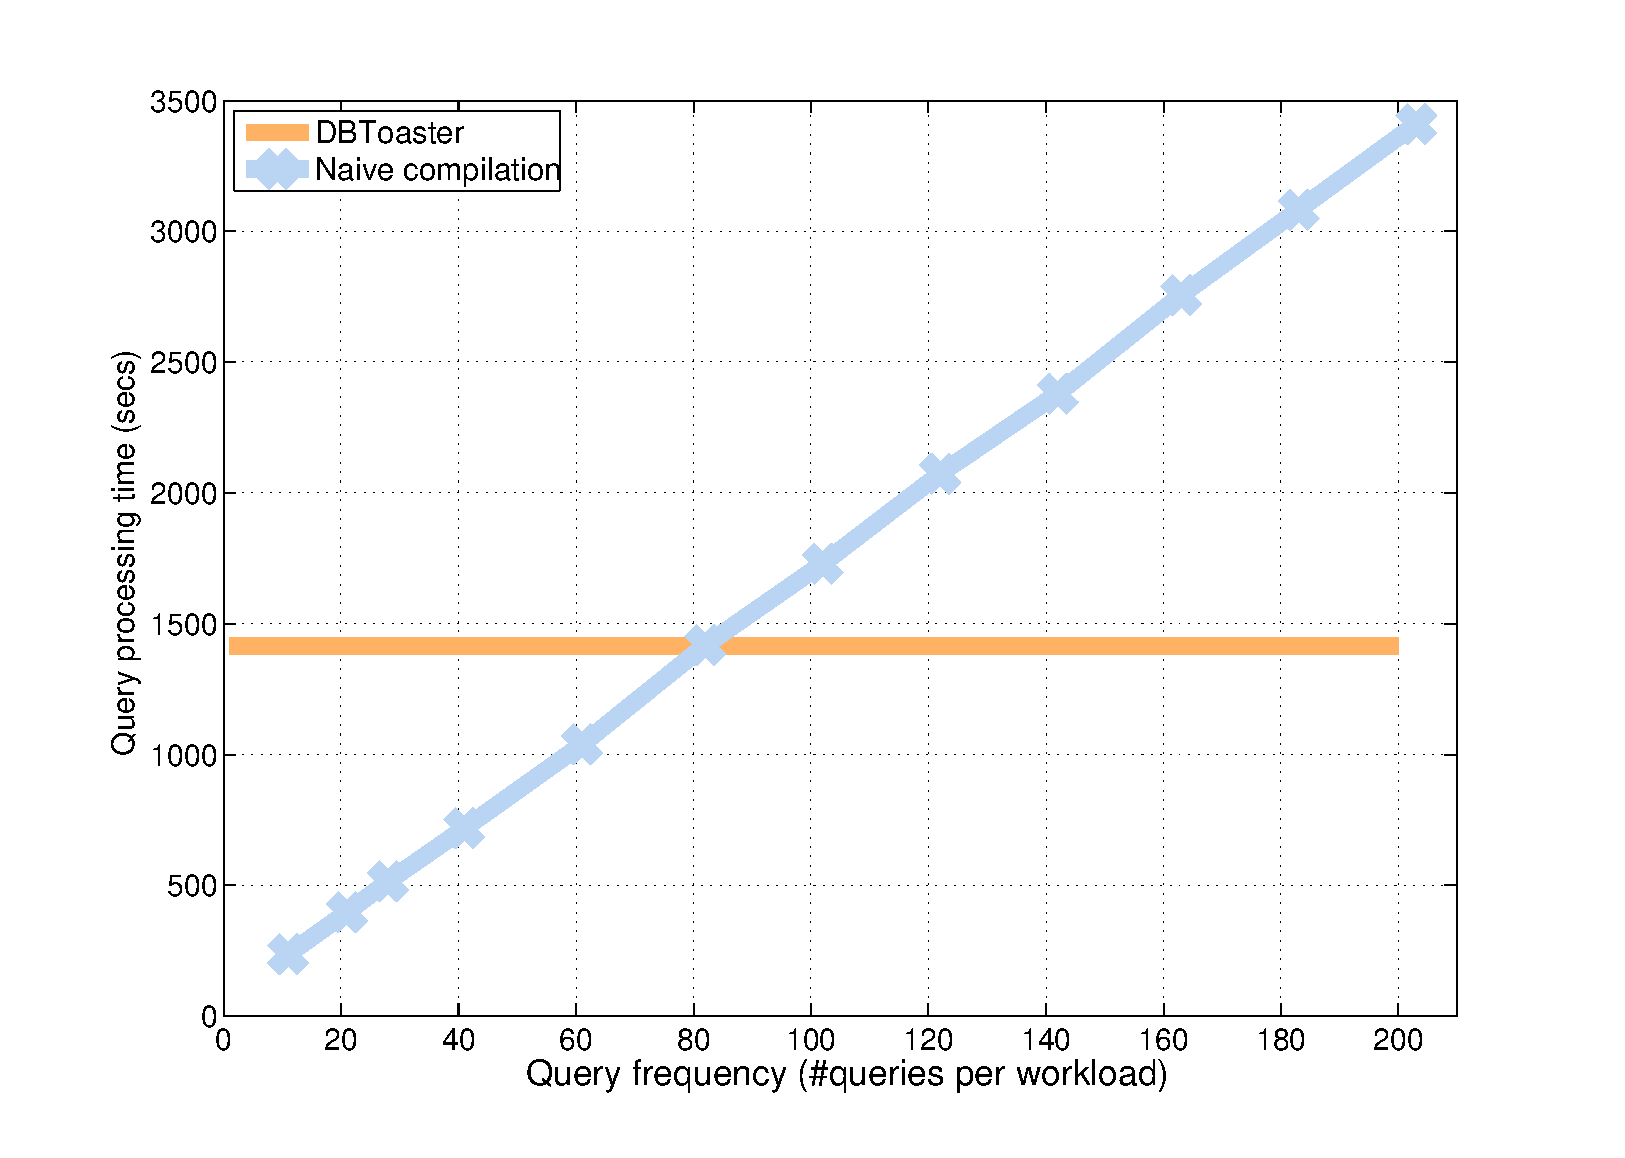
\includegraphics[scale=0.25]{../plots/vwap_query_freq_dn}
\end{center}
\caption{Query frequency limit for VWAP application, indicating the
query execution frequency beyond which DBToaster outperforms the naive query
plan compilation technique.}
\label{fig:vwap_query_freq}
\end{figure}

\begin{figure}
\begin{center}
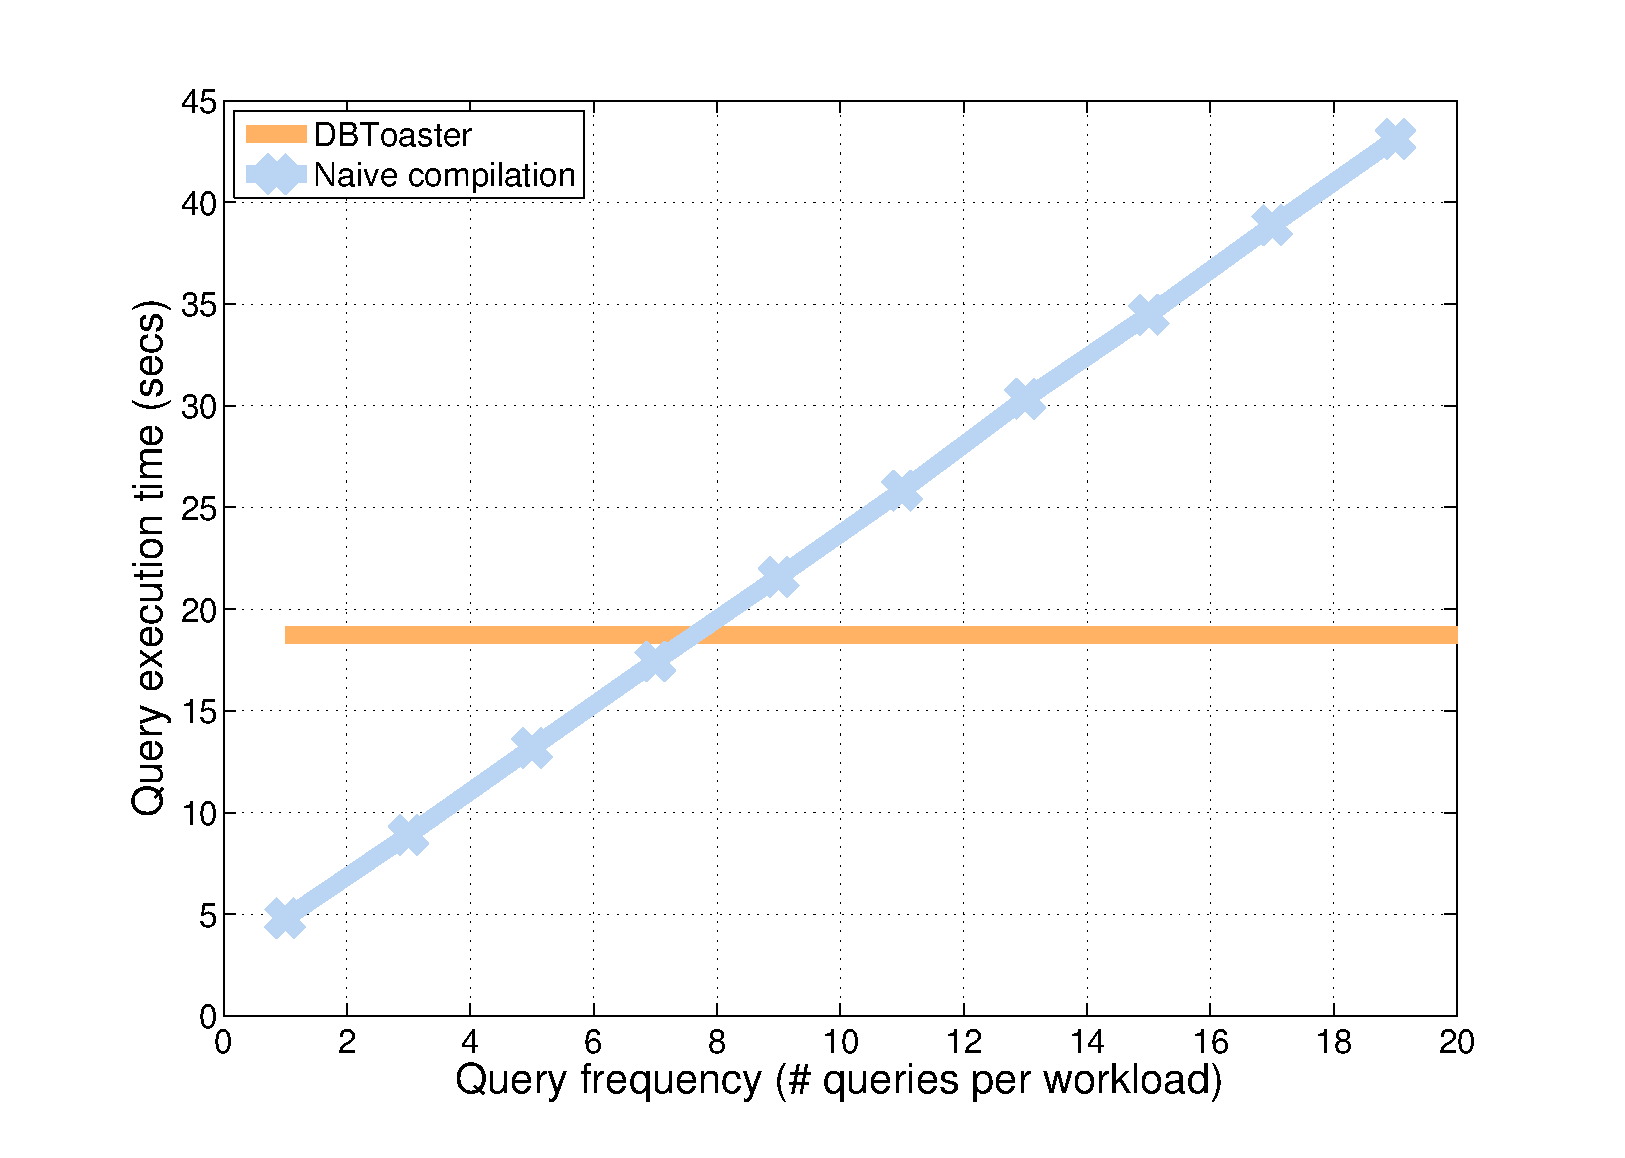
\includegraphics[scale=0.25]{../plots/ssb_query_freq_dn}
\end{center}
\caption{Query frequency limit for warehouse loading application, indicating the
query execution frequency beyond which DBToaster outperforms the naive query
plan compilation technique.}
\label{fig:ssb_query_freq}
\end{figure}

\subsection{Memory Analysis and Batch Execution}


\comment{
Dataset:

\begin{itemize}
  \item TotalView-ITCH dataset: 3 month's worth of MSFT order book messages
  taken from NASDAQ, (~2.2Gb dataset).
  \item Orderbook schema: day, time in us since beginning of day, order id,
  order type, share volume, bid/ask price
\end{itemize}

Queries:

\begin{verbatim}
select * from
  (select ax_bids.mmid, abs(
    sum(ax_bids.volume*
      (act_now.expected_price - ax_bids.price)) -
    sum(ax_asks.volume*
      (ax_asks.price - act_now.expected_price)))
    as ax_bias
  from
    (select mmid, price, volume from bids
       where mmid in axs) as ax_bids,
    (select mmid, price, volume from asks
       where mmid in axs) as ax_asks,
    (select expected_price
        from technical_indicator
        where entrance_condition)
    as act_now
  where ax_bids.mmid = ax_asks.mmid
  group by ax_bids.mmid) as sneaky_ax,
where ax_bias > 10000
\end{verbatim}

Figures:

\begin{enumerate}
  \item Takeaway experiment: end-to-end throughput comparison for a variety of
  insert/update/delete rates. Requires replay speed parameter in data loader.
  Comparison points include Postgres, naive compilation, simple version
  of \compiler, \compiler\ with lazy evaluation, \compiler\ with bulk insert
  mode at 2 or 3 different chunk sizes.

  \item Detail experiment: analyse effect of bulk loading operations compared to
  simple compiler, on a variety of queries, e.g. selectivities and keys.
  Dependent variables for plots: cache hit rates for locality analysis,
  throughput to understand pipelining effects. Is there anything lower lever we
  can do for pipelining?

  \item Detail experiment: selectivity experiment, comparing \compiler\ w/ lazy
  eval, and w/ bulk loading (separately) to next best, for a variety of
  join selectivities and keys.

  \item Detail experiment: space vs recomputation analysis, where we vary the
  maps we keep between extremes of maps from simple decomposition, to full base
  tables.

  \item Quality of compiled code, and compiler effect? e.g. speed provided with
  different -O flags?

\end{enumerate}
}

\section{Conclusion}

%\footnotesize{
\bibliographystyle{abbrv}%{plain}
\bibliography{sigmod12-dbtoaster,ref-long}
%}

\end{document}  

